
\documentclass[letterpaper]{article}
\usepackage{aaai}
\usepackage{times}
\usepackage{helvet}
\usepackage{courier}
\usepackage{graphicx}
\usepackage{amsmath}
\usepackage{tikz}
\usetikzlibrary{positioning, shapes.geometric, arrows.meta}
\usepackage{hyperref}


\frenchspacing
\setlength{\pdfpagewidth}{8.5in}
\setlength{\pdfpageheight}{11in}
\pdfinfo{
  /Title (Residual Network Architecture with Dynamic Data Augmentation, Squeeze-and-Excitation, and Stochastic Weight Averaging for Robust CIFAR-10 Image Classification)
  /Author (Humza, A., Zubairi, S.)
  
}
\setcounter{secnumdepth}{0}  

\begin{document}
\title{Residual Network Architecture with Dynamic Data Augmentation, Squeeze-and-Excitation, and Stochastic Weight Averaging for Robust CIFAR-10 Image Classification}
\author{Hamza, A., \& Zubairi, S. \\
Department of Electrical and Computer Engineering\\
New York University Tandon School of Engineering\\
\texttt{ah7072@nyu.edu | shz2020@nyu.edu}\\
\href{https://github.com/saadhzubairi/deep-learning-mini-projects}{Github Repository}
}
\maketitle
\begin{abstract}
\begin{quote}
We propose a compact ResNet for CIFAR‑10 that meets a 5M parameter constraint while achieving 95.31\% accuracy (Kaggle score 0.85485). Our design incorporates SE blocks, advanced regularization (dropout, label smoothing, stochastic depth), and dynamic data augmentation. A training strategy with warmup, cosine annealing, and SWA with BatchNorm freezing further optimizes performance.
\end{quote}
\end{abstract}
\section{Introduction}
CIFAR‑10 is a common benchmark with 60,000 32×32 color images in 10 classes. ResNets, known for their skip connections, ease the training of deep models. Here, we modify a ResNet to meet a 5M parameter limit while achieving state‑of‑the‑art performance on CIFAR‑10 by combining architectural enhancements, robust regularization, and optimized training techniques.

\section{Methodology}
\subsection{Architecture}
Our modified architecture builds upon a ResNet-18 foundation by enhancing its core residual block. In the traditional residual block, using the formulation \[ReLU(S(x)+F(x))\] as described in \cite{he2015deep} where S(x) is the identity skip connection and F(x) is a sequence of layers comprising a $3\times 3$ convolution, batch normalization, ReLU activation, followed by another $3\times 3$ convolution and batch normalization. In our design, we integrate Squeeze-and-Excitation (SE) blocks \cite{hu2018squeeze} immediately after the second convolution. These SE blocks perform global average pooling on the feature maps, then pass the resulting channel descriptors through a two-layer fully connected network (with a reduction ratio of 16) to learn channel-wise scaling factors. This adaptive recalibration of feature channels enhances representational power without significant parameter overhead.

Furthermore, we experimented with different residual block configurations, ultimately selecting a (3,3,2,1) block structure. The network starts with an initial convolution that maps the input image to 32 channels and progressively increases the number of channels (to 64, then 128, and finally 256) while reducing spatial dimensions via striding. An adaptive average pooling layer then aggregates spatial features into a fixed-size representation, which is fed into a final fully connected layer for classification into 10 classes.

This architectural design—combining a deeper block configuration, SE enhancements, and a balanced channel progression—enables the model to achieve high accuracy on CIFAR‑10 while remaining under the 5M parameter constraint.

\begin{figure}[ht]
\centering
\resizebox{0.9\linewidth}{!}{%
\begin{tikzpicture}[node distance=1.2cm, auto,
    block/.style={rectangle, draw, text width=3.5cm, align=center, rounded corners, minimum height=1cm},
    arrow/.style={-{Stealth}, thick}]

% Nodes
\node [block] (input) {Input\\$32\times32\times3$};
\node [block, right=of input] (conv) {Conv3x3, 32 filters\\BN + ReLU};
\node [block, right=of conv] (layer1) {Layer 1:\\3 Residual Blocks\\(with SE)\\Output: $32\times32\times64$};
\node [block, right=of layer1] (layer2) {Layer 2:\\3 Residual Blocks, Stride=2\\(with SE)\\Output: $16\times16\times128$};
\node [block, right=of layer2] (layer3) {Layer 3:\\2 Residual Blocks, Stride=2\\(with SE)\\Output: $8\times8\times256$};
\node [block, right=of layer3] (layer4) {Layer 4:\\1 Residual Block, Stride=2\\(with SE)\\Output: $4\times4\times256$};
\node [block, right=of layer4] (pool) {AdaptiveAvgPool2d\\$1\times1\times256$};
\node [block, right=of pool] (fc) {Dropout\\FC: 256 $\rightarrow$ 10};
\node [block, right=of fc] (output) {Output\\10 Classes};

% Arrows
\draw [arrow] (input) -- (conv);
\draw [arrow] (conv) -- (layer1);
\draw [arrow] (layer1) -- (layer2);
\draw [arrow] (layer2) -- (layer3);
\draw [arrow] (layer3) -- (layer4);
\draw [arrow] (layer4) -- (pool);
\draw [arrow] (pool) -- (fc);
\draw [arrow] (fc) -- (output);

\end{tikzpicture}
}
\caption{Final Modified ResNet Architecture with SE Blocks: Feature extraction through successive convolutional and residual layers, followed by global pooling and a classification head.}
\label{fig:resnet_architecture}
\end{figure}

\subsection{Training Methodology}

Our training strategy was designed to maximize generalization while respecting a 5M parameter constraint. In this section, we detail our key design choices, including hyperparameter tuning, optimization, regularization, and data augmentation.

\subsection{Hyperparameter Tuning}
We extensively tuned the architectural and training hyperparameters:
\begin{itemize}
    \item \textbf{Block Configuration and Network Depth:} We experimented with several ResNet variants. Our best configuration was ResNet (3,3,2,1), which increases the number of channels gradually from a base of 32 up to 256. All convolutions used 3$\times$3 kernels.
    \item \textbf{Channel and Kernel Sizes:} The network starts with 32 channels and progresses to 64, 128, and finally 256 channels, balancing expressiveness with parameter efficiency.
    \item \textbf{Batch Size and Total Epochs:} We primarily used a batch size of 128 and varied the total training duration from 35 to 150 epochs. Extended training (up to 150 epochs) allowed for better convergence and fine-tuning.
\end{itemize}

\subsection{Optimization}
We evaluated different optimizers and learning rate strategies:
\begin{itemize}
    \item \textbf{Optimizer Selection:} We compared SGD and AdamW. AdamW, \cite{loshchilov2019decoupled} with a learning rate of 0.003 and weight decay between 0.0007 and 0.00075, provided more stable convergence and superior generalization compared to SGD, which required a higher learning rate (around 0.01).
    \item \textbf{Learning Rate Scheduling:} Our learning rate schedule combined a warmup phase using LinearLR (starting at a factor of 0.01 for 5 iterations) with cosine annealing \cite{loshchilov2016sgdr} implemented via SequentialLR. The cosine annealing phase used a $T_{\text{max}}$ between 50 and 80 epochs and decayed the learning rate to an $\eta_{\text{min}}$ of approximately $1\times10^{-5}$.
    \item \textbf{Stochastic Weight Averaging (SWA):} To further enhance generalization, SWA \cite{izmailov2018averaging} was incorporated in the latter phase of training. Specifically, SWA was initiated at roughly 62.5\% of the total epochs (e.g., epoch 93 for a 150-epoch schedule) using an SWA learning rate between $3\times10^{-5}$ and $5\times10^{-5}$. This technique averages weights from multiple epochs to obtain a smoother, more robust final model.
\end{itemize}

\subsection{Regularization and Loss Settings}
To reduce overfitting, we applied multiple regularization techniques:
\begin{itemize}
    \item \textbf{Label Smoothing:}  \cite{szegedy2016rethinking} We experimented with label smoothing values of 0.0, 0.05, and 0.1. Label smoothing helps by softening the target labels and reducing the model's overconfidence.
    \item \textbf{Dropout:} Dropout was applied in the fully connected layers with rates between 0.1 and 0.35, which forces the network to learn redundant representations.
    \item \textbf{Stochastic Depth Dropout:} We incorporated stochastic depth dropout \cite{huang2016deep} (with probabilities of 0.0, 0.05, or 0.1) in the residual blocks. This technique randomly skips residual connections during training, encouraging the model to learn more robust features.
    \item \textbf{Squeeze-and-Excitation (SE) Blocks:} SE blocks were integrated within each residual block. They perform global average pooling followed by a two-layer fully connected network (with a reduction ratio of 16) to produce channel-wise scaling factors. This mechanism allows the network to recalibrate channel responses adaptively with minimal parameter overhead.
\end{itemize}

\subsection{Data Augmentation and Fine-Tuning}
We adopted a dynamic data augmentation strategy to further improve generalization:
\begin{itemize}
    \item \textbf{Early Training (Heavy Augmentation):} In the early phase, we used a heavy augmentation pipeline including:
        \begin{itemize}
            \item \textbf{RandAugment:} \cite{cubuk2020randaugment} Applied with 3 operations at a magnitude of 9.
            \item \textbf{ColorJitter:} Adjusting brightness, contrast, and saturation by 0.2 and hue by 0.1.
            \item \textbf{Random Erasing:} \cite{zhong2017random} With a probability of 0.1--0.2 to simulate occlusions.
        \end{itemize}
        In addition, we applied MixUp \cite{zhang2018mixup} and CutMix \cite{yun2019cutmix} augmentation:
        \begin{itemize}
            \item \textbf{MixUp:} Blending two images using a mixing coefficient sampled from a Beta distribution with an alpha value of 0.2 or 0.4.
            \item \textbf{CutMix:} Replacing a region of one image with a patch from another, using an alpha value of 1.0.
        \end{itemize}
        These augmentations were applied with a 35\% probability during early epochs to promote robustness.
    \item \textbf{Fine-Tuning Phase:} During the final 25\% of epochs, we transitioned to a lighter augmentation pipeline that consisted of basic random cropping, horizontal flipping, and normalization. Concurrently, the probability of applying MixUp/CutMix was reduced to 15\% to allow the model to refine its decision boundaries on less perturbed data. Furthermore, BatchNorm layers were frozen in the final epochs (starting around 87.5\% of total epochs) to stabilize normalization statistics.
\end{itemize}

Together, these strategies enabled our modified ResNet to achieve high test accuracy on CIFAR-10 while remaining within the 5M parameter constraint. Each component—from architectural adjustments to the dynamic augmentation and SWA—played a crucial role in enhancing the model's generalization performance.

\section{Iterative Model Improvements}

From the original ResNet-18 architecture described in \cite{he2015deep}, we made several modifications to improve performance while adhering to a 5M parameter constraint. Our evolution can be summarized as follows:

\begin{enumerate}
    \item \textbf{Model 1: Baseline.} Standard ResNet (2,2,2,2) with 2.7M parameters, trained using SGD (LR=0.01, WD=0.0005) and advanced augmentation (random cropping, flipping, ColorJitter). Minimal regularization yields 88.3\% accuracy (Kaggle: 0.76536). See Figure~\ref{fig:training_performance_8825}.
    
    \begin{figure}[ht]
    \centering
         \includegraphics[width=0.7\linewidth]{images/traintest_lost-88.25.png}
    \caption{Train/test loss over 35 epochs (Model 1).}
    \label{fig:training_performance_8825}
    \end{figure}

    \item \textbf{Model 2: Regularization Improvements.} Introducing label smoothing (0.05--0.1) and increasing dropout (up to 0.35) improves accuracy to 89.8\% (Kaggle: 0.78232).

    \item \textbf{Model 3: Augmentation \& Architecture Change.} Switching to a ResNet (2,2,2,1) and applying MixUp and CutMix (35\% probability) with SWA starting after 30 epochs yields approximately 89.4\% accuracy (Kaggle: 0.77075).

    \item \textbf{Model 5: Optimizer \& Tuning.} Using AdamW (LR=0.003, WD$\approx$0.0007–0.00075), reducing label smoothing (0.05), increasing dropout (0.35), and starting SWA earlier (after 25 epochs) raises accuracy to 92.70\% (Kaggle: 0.81584).

    \item \textbf{Models 6--8: Minor Tweaks.} Further refinements—such as a deeper ResNet (3,3,2,1) with no label smoothing, moderate dropout (0.2), and fine-tuning with AdamW (LR=0.01)—yield accuracies of 93.18\% and 94.06\% (Kaggle: 0.82482 and 0.82621), which are combined in our narrative.

    \item \textbf{Model 9: SE Blocks Integration.} Incorporating SE blocks (reduction ratio=16), reducing dropout (0.1), and maintaining label smoothing (0.1), with SWA starting after 50 epochs, increases accuracy to 94.62\% (Kaggle: 0.84497). See Figure~\ref{fig:training_performance_9462}.
    
    \begin{figure}[ht]
    \centering
         \includegraphics[scale=0.3]{images/train_test_loss_94.62.png}
    \caption{Train/test loss over 80 epochs (Model 9).}
    \label{fig:training_performance_9462}
    \end{figure}

    \item \textbf{Model 10: Final Model.} Extending training to 150 epochs, using lighter augmentation in the final 25\% (MixUp/CutMix probability reduced to 15\%), freezing BatchNorm layers in the final 10\% (from epoch 131), and starting SWA at 62.5\% (epoch 93) with SWA LR of $5\times10^{-4}$, the final model achieves 95.31\% accuracy (Kaggle: 0.85485). See Figure~\ref{fig:training_performance}.
    
    \begin{figure}[h]
    \centering
        \includegraphics[width=0.9\linewidth]{images/train_test_loss_95.31.png}
    \caption{Train/test loss over 150 epochs (Model 10).}
    \label{fig:training_performance}
    \end{figure}
\end{enumerate}

These changes increased the accuracy to 95.31\% and the Kaggle score to \textbf{0.85485}.

This evolution demonstrates how systematic modifications to architecture, regularization, and training strategies collectively enhanced our model's performance and generalization on CIFAR-10. The iterative model accuracy improvements can be seen in \ref{fig:all_iterations}

\begin{figure}[ht]
\centering
\includegraphics[width=0.8\linewidth]{images/accuracy_charts.png}
\caption{Training performance over successive model iterations showing progressive improvements in accuracy and kaggle score.}
\label{fig:all_iterations}
\end{figure}

\section{Observations and Analysis}

\subsection{Training Dynamics}
Figure~\ref{fig:training_performance} shows the evolution of training and validation losses over 150 epochs. Early in training, aggressive data augmentation (RandAugment, ColorJitter, Random Erasing, MixUp, and CutMix) drives a rapid decrease in loss. In later epochs, a transition to a lighter augmentation scheme stabilizes the gradients and reduces noise, indicating effective fine-tuning and convergence.

    \subsection{Ablation Studies}
Our systematic ablation experiments reveal the impact of individual design choices:
\begin{itemize}
    \item \textbf{SWA and BatchNorm Freezing:} Activating Stochastic Weight Averaging (SWA) from 62.5\% of the training, together with freezing BatchNorm layers in the final 10\%, results in smoother loss curves and improved generalization. Omitting either technique increases variance and degrades performance.
    \item \textbf{Regularization Techniques:} The combined use of dropout, stochastic depth, and label smoothing effectively minimizes overfitting. Removing any one of these methods causes a larger gap between training and validation losses.
\end{itemize}

These analyses confirm that each component—when applied individually or in combination—contributes significantly to robust convergence and improved generalization.



\subsection{Confusion Matrix Analysis}
To further assess class-level performance, we visualize the confusion matrix in Figure~\ref{fig:conf_matrix}. The strong diagonal dominance indicates the model accurately classifies most examples within each class. However, certain classes (e.g., \emph{cat} and \emph{dog}) exhibit minor confusion, reflecting their visual similarity at low resolution. Understanding these misclassifications can guide targeted augmentations or specialized fine-tuning strategies for even better results.
\begin{figure}[ht]
    \centering
    \includegraphics[width=0.8\linewidth]{images/conf_matrix.png}
    \caption{Confusion matrix for the final model on the CIFAR-10 test set. Diagonal dominance shows robust class performance, with minor off-diagonal entries indicating occasional misclassifications.}
    \label{fig:conf_matrix}
\end{figure}

\subsection{Conclusion}
We present a compact Residual Network that achieves state-of-the-art CIFAR‑10 performance with only 4.4 million parameters. Our final model reaches a Kaggle score of \textbf{0.85485} (95.31\% accuracy), proving that strategic architectural and training innovations can yield robust performance within a tight parameter budget. Key drivers include:
\begin{itemize} 
    \item \textbf{Modified Architecture:} A compact ResNet with Squeeze-and-Excitation blocks for dynamic channel recalibration.
    \item \textbf{Advanced Regularization:} The combined use of FC dropout, stochastic depth, and label smoothing to mitigate overfitting.
    \item \textbf{Dynamic Data Augmentation:} An aggressive early-stage augmentation strategy that transitions to a lighter scheme during fine-tuning.
    \item \textbf{Optimized Training Strategy:} AdamW with a warmup phase, cosine annealing, and SWA to enhance convergence and stability.
\end{itemize}
\begin{table}[h]
\centering
\begin{tabular}{lccc}
\hline
\textbf{Variant} & \textbf{Accuracy (\%)} & \textbf{Kaggle Score} \\
\hline
Baseline  & 88.3 & 0.76536 \\
+ Regularization &  89.8 & 0.78232 \\
+ Data Augmentation  & 89.4 & 0.77075 \\
+ AdamW + SWA  & 92.7 & 0.81584 \\
+ Architecture Change & 94.06 & 0.8261\\
+ SE Blocks &  94.6 & 0.84497 \\
Final Model & \textbf{95.31} & \textbf{0.85485} \\
\hline
\end{tabular}
\caption{Performance evolution across model iterations.}
\label{tab:results_summary}
\end{table}
Table~\ref{tab:results_summary} summarizes the performance evolution, highlighting the cumulative benefits of these design choices. Our results demonstrate that even under a 5M parameter constraint, systematic tuning and strategic model design can achieve competitive, real-world performance, setting a new benchmark for efficient deep learning on CIFAR‑10.

\bibliographystyle{aaai}  % or your preferred bibliography style
\bibliography{references}


\end{document}